\documentclass[a4paper]{jpconf}
\usepackage{graphicx}
\begin{document}
\title{Exploiting analytics techniques in CMS computing monitoring}

\author{D Bonacorsi$^1$, V Kuznetsov$^2$, N Magini$^3$, A Repe\v{c}ka$^4$ and E Vaandering$^3$}

\address{$^1$ Universit\`a di Bologna, Bologna, Italy}
\address{$^2$ Cornell University, Ithaca, NY, USA}
\address{$^3$ Fermi National Accelerator Laboratory, Batavia, IL, USA}
\address{$^4$ University of Vilnius, Vilnius, Lithuania}

\ead{bonacorsi@bo.infn.it, vkuznet@gmail.com, Nicolo.Magini@cern.ch, aurimas.repecka@mif.stud.vu.lt, ewv@fnal.gov}

\begin{abstract}
The CMS experiment has collected an enormous volume of metadata about its computing operations in its monitoring systems, describing its experience in operating all of the CMS workflows on all of the Worldwide LHC Computing Grid Tiers. Data mining efforts into all these information have rarely been done, but are of crucial importance for a better understanding of how CMS did successful operations, and to reach an adequate and adaptive modelling of the CMS operations, in order to allow detailed optimizations and eventually a prediction of system behaviours. These data are now streamed into the CERN Hadoop data cluster for further analysis. Specific sets of information (e.g. data on how many replicas of datasets CMS wrote on disks at WLCG Tiers, data on which datasets were primarily requested for analysis, etc) were collected on Hadoop and processed with MapReduce applications profiting of the parallelization on the Hadoop cluster. We present the implementation of new monitoring applications on Hadoop, and discuss the new possibilities in CMS computing monitoring introduced with the ability to quickly process big data sets from mulltiple sources, looking forward to a predictive modeling of the system.
%CMS experiment highly depends on data and even more of metadata analysis. This paper suggests to concentrate on specific CMS data data analysis - dataset block replica storage occupation. 
%This paper provides fully-covered approach for analysis process. It contains of four main segements: reading data, processing data, writing and visualizing results. Most of the decisions 
%made in the approach were chosen in order to get high configurability and good performance. Created service takes advatage of Hadoop, Spark, Elasticsearch and Kibana technologies.
\end{abstract}

\section{Introduction}
The CMS experiment \cite{CMS} produces a huge amount of data: currently more than 150 PB of CMS data are replicated among the centres of the Worldwide LHC Computing Grid \cite{WLCG}. Different sets of metadata about these data are recorded in the CMS computing services to control workflows on the Grid.
Data mining efforts on the computing metadata are of crucial importance to see how 
CMS did succesful operations and to allow optimizations and system behaviour predictions. This paper concentrates on the analysis of a specific set of information: storage space occupation by dataset block replicas.

CMS data are recorded in files which are organized in datasets and blocks. Datasets are sets of files with common physics content, and have a size ranging from a 
few files and few GBs to several hundred thousand files and hundreds of TBs depending on the physics definition. Datasets are divided into groups of files called blocks to simplify data management; each block has a typical size of 100-1000 files and 100 GB-1 TB \cite{DMWM}. The CMS data management system PhEDEx \cite{PhEDEx} distributes the data to tens of sites and tracks in its Oracle database the location of every replica of every block produced by CMS. In addition to the site where the replica is stored, PhEDEx records several additional metadata about each block replica, including:

\begin{itemize}
\item Dataset to which the block belongs. From the dataset name, the {\it acquisition era} when the data were produced and the {\it data tier} (i.e. data format, e.g. RAW or RECO) can be deduced.
\item Number and size of files in the block replica which are resident on, produced at, transferring to and subscribed to the site storage,
\item Type of site storage, i.e. disk or tape,
\item Custodiality of the block replica, i.e. whether the site has the responsibility to 
preserve an archival copy of the files on tape,
\item Group of users which requested the placement of the replica at the site.
\end{itemize}

The PhEDEx database keeps only the current status of the block replicas, and some high-level historical aggregations. Therefore, it is not possible to perform a detailed historical analysis of the evolution of storage space occupied by the replicas of different types of CMS data using PhEDEx alone.

For this reason, in 2015 we started to export daily snapshots of the PhEDEx block replica information to a Hadoop file system to preserve the historical evolution of space occupation.

Taking advantage of the technologies offered in the analytics ecosystem, in 2016 we built a fully-covered service to analyse these monitoring data. In this paper, we present this effective and flexible approach to analyse and visualize the storage occupation of block replicas.

The system consists of four main segments: reading data, processing data, storing results and visualizing results. Most of the technology choices were made in order to get high flexibility and good performance. 
The basic structure of the monitoring system is shown in figure \ref{fig:structure}, together with the technologies used for each step: Hadoop, Spark, Elasticsearch and Kibana.
With this architecture, we can efficiently perform all sorts of new analyses on the replica monitoring information without adding any load on the live PhEDEx service in Oracle.

\begin{figure}[t]
\begin{center}
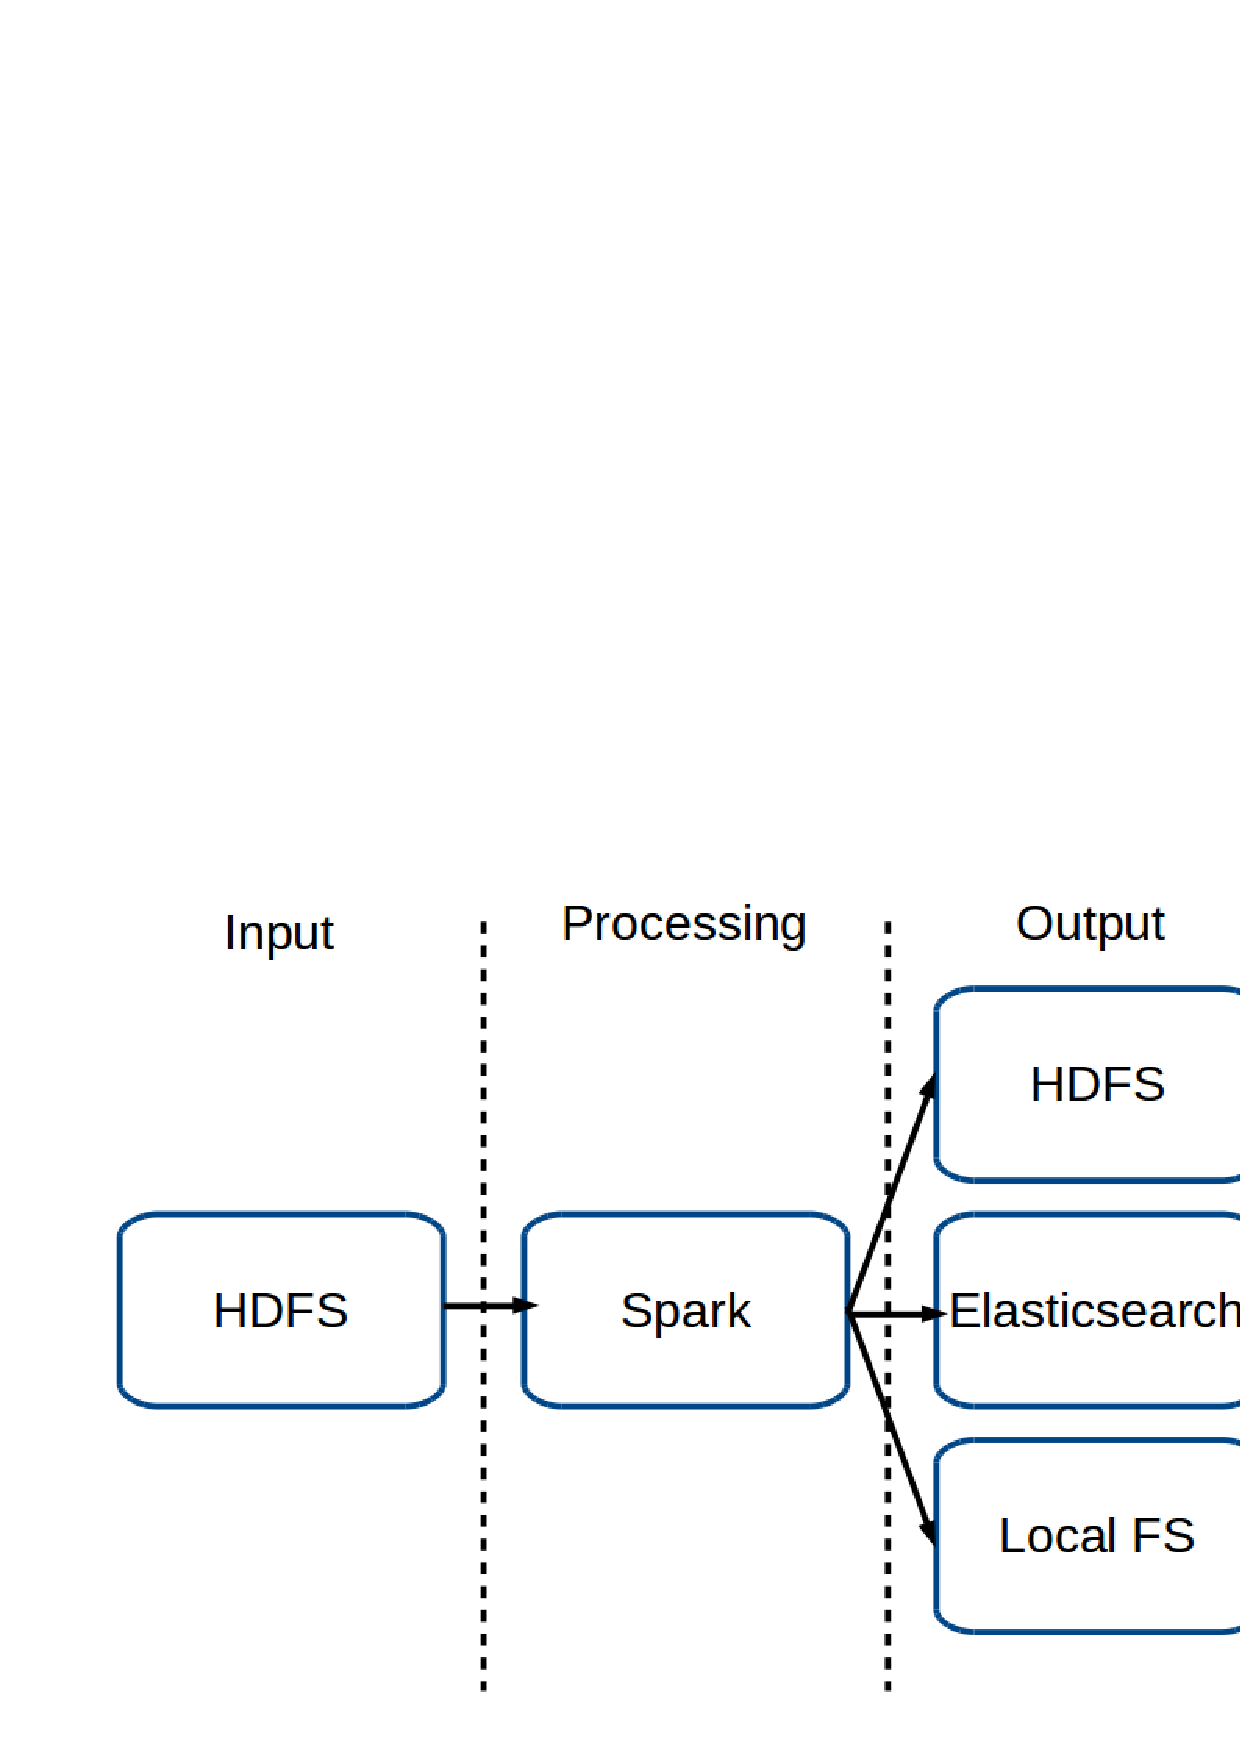
\includegraphics[width=15cm]{structure.png}\hspace{2pc}%
\caption{\label{fig:structure}Structure of the CMS dataset block replica monitoring system}
\end{center}
\end{figure}


\section{Input and processing}

Every day, a snapshot of the block replica information is exported with Sqoop \cite{Sqoop} from the PhEDEx Oracle database to the \textit{analytix} Hadoop cluster hosted by CERN IT. The \textit{analytix} cluster is composed by 38 heterogeneous nodes, with 2 TB of total memory, about 1000 virtual CPU cores allocated to run jobs, and nearly 2 PB of raw storage. CPU time and disk space are shared among CERN users according to quotas.

Block replica data snapshots exported with Sqoop are stored as CSV files with a fixed schema, and have a size ranging from 2 GB to 3.5 GB, increasing with the growth of CMS data. As a long term solution, we chose to keep these data in the Hadoop Distributed File System (HDFS) \cite{Hadoop}, which provides the advantages of scalability, effectiveness and resilience to failure.
 

Block replica snapshots contain many informative fields (e.g. block size, replica location, user group who requested the data, etc.) which cannot be analysed all at once. In addition, some of the input fields need to be processed to derive additional required information: for example, data tier and acquistion era need to be parsed from the dataset name.
 To fix this issue, the system had to provide a means of reducing data dimensions and simplify the data dropping useless fields while producing the needed ones.
 
 
Dynamic aggregation is the core of this approach, allowing us to reduce data complexity for every service execution. The service allows to define one or more grouping keys, one or more result values, and the aggregation function to use for each result value. Aggregations include basic operations such as sum, count, min, max, first, last, mean.
For more complicated analyses, two extra operations were implemented: a daily time-average, 
which simply calculates the sums of every result field and divides each of them by the number of days analysed, and a delta operation computing the growth and decrease of each result in a customizable time period (to measure e.g. the total amount of data written to and deleted from a site during that period).

We also implemented data ordering and data filtering (by one or more fields), using regular expressions to filter text fields.
In this way we are able to reduce the amount of non-informative information to 
a minimum, caching in memory only the subset of data of interest.

The dynamic aggregation and filters are fully configurable: this means that implementing a new analysis on the data is simply a matter of configuring the service to run with new parameters, adding a lot of flexibility to the system.

As efficiency was one of the main goals of the approach, to implement the processing module the Spark \cite{Spark}  technology was chosen. Spark, provided on the \textit{analytix} cluster as user tool, is a framework for distributed data processing that, unlike Map\&Reduce, tries to cache data in memory in order to reuse them as much as possible, minimizing disk IO operations.
Dataframes \cite{Dataframes} and sparkSQL were used instead of Spark RDDs to achieve better performance. All of the algorithms in the aggregation process were implemented in a manner that reduces data shuffling as much as possible, to avoid the performance hit incurred moving large amounts of data through the network.

\section{Result output}

The service provides a few different options to store the results; each of them is best suited for a specific purpose.
\begin{itemize}
\item Hadoop file system. It should be used for long-term storage and for large result sets.
\item Local file system. It should be used for quick aggregations stored in a personal environment. The aggregation level should be chosen appropriately in order to get small files. This option can consume a large amount of memory on the master node where the data need to be collected for output.
\item Elasticsearch resource \cite{Elasticsearch}. It should be used to store in the Elasticsearch search engine the results that need to be visualized.
\end{itemize}

The Elasticsearch output module is the main mode of operation of the block replica monitoring. 
Using a third-party package \cite{Elasticsearchspark}, we could make a direct connection from Spark to Elasticsearch without the need for an extra step. When writing data to Elasticsearch, an extra field "origin" is added to the schema. Since the service can be run for different purpouses (cronjob or custom execution), the extra field helps to keep the results of different processes separate for analysis and visualization.


To keep the replica monitoring system modular, the node, port and resource (index/type) of the Elasticsearch service can be fully configured; currently we are using Elasticsearch running on a privately deployed server, but we are planning to migrate the service to write to the Elasticsearch service provided by the CERN IT monitoring team \cite{itmon}.

\section{Performance}

Having a good performance for data processing was one of the most important goals of this approach. In addition to running the processing in parallel with YARN, we applied several optimizations to reduce processing time to a minimum, and we measured the related performance improvements. As different aggregations have different performance results, we provide performance figures for two different aggregations: sum, which is considered to be a low-cost operation, and delta, which is 
considered to be a computationally expensive operation. Allocated resources (not necessarily used) are written in the 
performance tables \ref{tab:performance-sum} and \ref{tab:performance-delta}.


\begin{table}[t]
\begin{center}
\caption{Performance of basic aggregations}
\label{tab:performance-sum}
\begin{tabular}{l*{6}{c}r}
\br
Interval 	   & Input	     & Cores	      & Memory 		& Output 	  & Duration \\
\mr
1 day              & ~3 GB            & 65             & 361472 MB        & ~600 kB          & ~1.6 min \\
1 month            & ~100 GB          & 65             & 361472 MB        & ~18 MB           & ~4.3 min \\
3 months           & ~310 GB          & 65             & 361472 MB        & ~52 MB  	  & ~9.7 min \\
1 year             & ~1.1 TB          & 65             & 361472 MB        & ~186 MB          & ~28 min \\
\br
\end{tabular}

Group keys: now, user group, acquisition era, data tier, node kind

Result fields: node bytes, destination bytes

Aggregations: sum, sum

Output: Hadoop file system
\end{center}
\end{table}
\begin{table}[t]
\begin{center}
\caption{Performance of delta aggregations}
\label{tab:performance-delta}
\begin{tabular}{l*{6}{c}r}
\br
Interval	   & Input	     & Cores	      & Memory		& Output 	  & Duration \\
\mr
2 days             & ~5 GB            & 65             & 361472 MB        & ~12.7 kB         & ~2.5 min \\
7 days             & ~20 GB           & 65             & 361472 MB        & ~41.6 kB         & ~4 min \\
1 month            & ~90 GB           & 65             & 361472 MB        & ~189.2 kB  	  & ~8.5 min \\
6 months           & ~500 GB          & 65             & 361472 MB        & ~1 MB            & ~35 min \\
\br
\end{tabular}

Group keys: now, node name

Result fields: node bytes

Aggregations: delta (interval 1 day)

Output: Hadoop file system

\end{center}
\end{table}

\section{Visualization}

The structure of the analysis service allows to reduce the complexity of the visualization process to a minimal level. With the results stored in an Elasticsearch resource, we can use the visualization technologies built on top of it. In particular, we chose to use Kibana \cite{Kibana} to build the visualization layer, so that we only needed to create the Kibana configuration without writing any code.
Then the operators performing the analysis can define searches themselves, create visualizations of current and historical data, and compose dashboards according to their own needs.
One of the example visualizations created with Kibana can be seen in figure \ref{fig:pie-charts}. This chart simply shows the 10 acquisition eras which are currently consuming the most storage space, separately for two user groups which requested the data (AnalysisOps, DataOps).

\begin{figure}[t]
\begin{center}
\includegraphics[width=15cm]{pie-charts.png}\hspace{2pc}%
\caption{\label{fig:pie-charts}Kibana visualization of current block replica data}
\end{center}
\end{figure}

Another example is shown in figure \ref{fig:bar-charts}. This chart shows the time evolution of the 10 data tiers which consumed the most storage space.

\begin{figure}[t]
\begin{center}
\includegraphics[width=15cm, height=7cm]{bar-charts.png}\hspace{2pc}%
\caption{\label{fig:bar-charts}Kibana visualization of historical block replica data}
\end{center}
\end{figure}

\section{Conclusions}

We developed an analysis service to reduce dimensions (aggregation) and visualize block replica monitoring data.
The approach used has three main advantages. First of all, it is very efficient as it is build on top of Spark which allows distributed computing in memory without disk access.
In addition, the service is fully-covered, with the possibility to get everything from the raw data in the Hadoop file system to visualizations and dashboards in Kibana.
Finally, the system is highly configurable. If there is a need to look at 
data from a different perspective, the operators only need to change the service parameters for the job executions. This results in different aggregations, different results written in the Hadoop file system and Elasticsearch, and different visualizations and dashborads in Kibana, without changing the service itself.

We have already started to use the block replica monitor to produce custom aggregations for computing reports, and we have now set up the first basic cron processes to produce historical plots for operators. We are now planning to expand the service with more standard aggregations, and to migrate the output to the CERN IT Elasticsearch+Kibana service where the operators can define the visualization dashboards most suited to their needs.


\section*{References}
\medskip
\begin{thebibliography}{9}
\bibitem{CMS} The CMS collaboration 2008 The CMS experiment at the CERN LHC {\it JINST} {\bf 3} S08004
\bibitem{WLCG} Eck C {\it et al.} 2005 LHC Computing Grid Technical Design Report {\it CERN-LHCC-2005-024}
\bibitem{DMWM} Giffels M, Guo Y, Kuznetsov V, Magini N and Wildish T 2014 The CMS Data Management System {\it J. Phys.: Conf. Ser.} {\bf 513} 042052 
\bibitem{PhEDEx} Egeland R, Metson S and Wildish T 2008 Data transfer infrastructure for CMS data taking. {\it XII Advanced Computing and Analysis Techniques in Physics Research (Erice, Italy: 
Proceedings of Science)}
\bibitem{Sqoop} http://sqoop.apache.org/
\bibitem{Hadoop} http://hadoop.apache.org/ 
\bibitem{Spark} http://spark.apache.org/
\bibitem{Dataframes} https://databricks.com/blog/2015/02/17/introducing-dataframes-in-spark-for-large-scale-data-science.html
\bibitem{Elasticsearch} https://www.elastic.co/products/elasticsearch
\bibitem{Elasticsearchspark} https://www.elastic.co/products/hadoop 
\bibitem{itmon} Aimar A 2016 Unified Monitoring Architecture for IT and Grid Services, CHEP 2016
\bibitem{Kibana} https://www.elastic.co/products/kibana
\end{thebibliography}
\smallskip

\end{document}


